
\documentclass[10pt,letterpaper,unboxed,cm]{article}
\usepackage[margin=1in]{geometry}
\usepackage{graphicx}
\usepackage{enumerate}

\newcommand{\st}{~\mid~}
\newcommand{\ind}{$~~~$}
\usepackage{xcolor}

\graphicspath{ {./../images} }
\begin{document}


\hfill{CSE 101 Spring 2024}
\hfill{Homework 1}
\hfill{Due: Wednesday 4/10 at 11:59pm}

\begin{enumerate}

%FIRST PROBLEM

\item (10 points)\\
\emph{[The purpose of this problem is to review a few concepts we will need in this class: asymptotic notation, recurrence relations and induction]}

Let $T$ be defined by the recurrence relation:
$$T(0) = 1~,T(1) = 4~~~~~~~ T(n) = T(n-1) + 2T(n-2) + (3)(2^{n-1})~~for~~all~~n\geq 2$$

\begin{enumerate}
\item
Prove that $T(n)=\Omega(2^n)$ using induction.

\item
Prove that $T(n) = O(n2^n)$ using induction.

\end{enumerate}



% SECOND PROBLEM



\item (12 points)

\emph{[This problem is designed to give a concrete example of a graph with $n$ vertices such that the number of paths grows faster than any exponential (in terms of $n$). This is important later when we start looking for paths with specific properties (shortest paths, paths of even or odd length, paths that avoid certain vertices, etc.) Some of you will be tempted to say ``Search all paths....." but this may require a runtime that grows exponentially or faster. It is important to note that DFS, BFS,... do not search all paths since these algorithms are polynomial time.]}

Let $B(n)$ be the $n$th \emph{Complete Balanced Bipartite Graph} on $2n$ vertices. $B(n)$ has $2n$ vertices $n$ on each side. One side has vertices labeled $a_1,\dots,a_n$ and the other side has vertices labeled $b_1,\dots,b_n$. There is an edge connecting $a_i$ and $b_j$ for all $1\leq i,j\leq n$

Below is the graph of $B(3):$

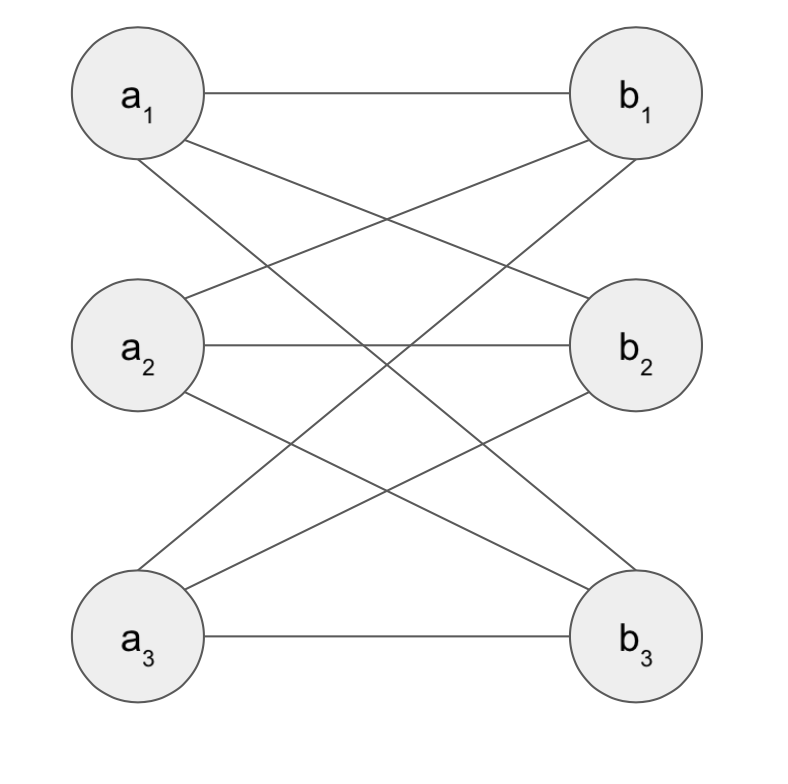
\includegraphics[scale = 0.2]{Bipartite.png}


\begin{enumerate}
\item
How many edges does $B(n)$ have? (no justification necessary)
\item
Let $H(n)$ be the number of Hamiltonian paths of $B(n)$  that start from an $a_i$ vertex and ends at a $b_j$ vertex (Hamiltonian paths are paths that go through each vertex exactly once.)

Give an explanation as to why $H(n) = (n!)^2$

\item
Let $P(N)$ be the number of Hamiltonian paths of a Complete Bipartite Graph on $N$ vertices. Determine the big-Theta bound of $P(N)$.
\end{enumerate}

\item (15 points)\\
\emph{[This main motivation for this problem is to see that if the graph is given to you in a matrix form, you may be able to use matrix operations to answer certain questions.]}


A {\em triangle}  in an undirected, simple graph is a set of three 
distinct vertices $x, y, z$ such that all pairs are connected by an edge. 

\begin{enumerate}
\item
Consider the following algorithm that takes as input an adjacency matrix of a simple undirected graph $G$ and returns True if there exists a triangle and returns False if there is not a triangle.

\begin{quote}
\emph{Triangle1}$(G)$ ($G$, an undirected simple graph with $n$ vertices in adjacency matrix form.)
\begin{enumerate}[1.]
\item
{\bf for} $i = 1,\dots, n$:
\item
\ind {\bf for} $j = 1,\dots, n$:
\item
\ind \ind {\bf if} $G[i,j] == 1:$
\item
\ind\ind\ind {\bf for} $k = 1,\dots, n$:
\item
\ind\ind\ind\ind {\bf if} $G[i,k] == 1$ and $G[j,k] == 1$:
\item
\ind\ind\ind\ind\ind {\bf return} True
\item
{\bf return} False
\end{enumerate}
\end{quote}

(3 points)
Show that the runtime for this algorithm is $O(|V|^2 +|V||E|)$.

\item (3 points)
In order for \emph{Triangle1} to return True, what needs to happen and why does this correspond to a triangle?


\item 
Consider the following algorithm that takes as input an adjacency matrix of a simple undirected graph $G$ and returns True if there exists a triangle and returns False if there is not a triangle.

\begin{quote}
\emph{Triangle2}$(G)$ ($G$, an undirected simple graph with $n$ vertices in adjacency matrix form.)
\begin{enumerate}[1.]
\item
Compute $H = G \times G$.
\item
{\bf for} $i = 1,\dots, n$:
\item
\ind {\bf for} $j = 1,\dots,n$:
\item
\ind\ind {\bf if} $G[i,j] == 1$ AND $H[i,j] > 0$:
\item
\ind\ind\ind {\bf return} True
\item
{\bf return} False
\end{enumerate}
\end{quote}

(3 points)
Assuming that matrix multiplication between two $n\times n$ matrices takes $O(n^{2.81})$ time, calculate the runtime of this algorithm. 

\item
(3 points)
In order for \emph{Triangle2} to return True, what needs to happen and why does this correspond to a triangle? (In particular, what does it mean for $H[i,j] = 1$ or $H[i,j] = 2$?)

\item
(3 points)
Is \emph{Triangle1} or \emph{Triangle2} more efficient? (Justify your answer.) (Hint: think about dense and sparse graphs.)
\end{enumerate}




%FOURTH PROBLEM
\item (10 points) \\
\emph{[The main motivation for this problem is to see what a \emph{reduction} algorithm looks like. Also, in this problem, you will practice writing a bi-directional proof for an algorithm that solves a decision problem.]}\\
Given a directed graph $G$ with vertex weights $w_v\in\{0,1,2\}$ (in other words, each vertex is either labeled with 0,1 or 2), and vertices $s$ and $t$, 
Determine if there is a path in $G$ from $s$ to $t$ such that the ternary sequence of vertex weights in the path does not repeat the same number twice in a row.

Consider the following algorithm that claims to solve this problem: 

\begin{quote}
{\bf Algorithm Description:}

Input: a $\{0,1,2\}$-labeled directed graph $G$, a vertex $s$ of $G$ and a vertex $t$ of $G$.

Create a graph $G'$ by removing all edges $(u,v)$ such that $w(u) == w(v)$.

Run graphsearch on $G'$ starting from $s$. If $t$ is visited then return TRUE. Otherwise return FALSE

\end{quote}




(NOTE: \emph{graphsearch} is an algorithm that takes a graph $G$ and a vertex $s$ and returns a list of vertices that are reachable from $s$ by a directed path in $G$.
You do not have to prove the correctness of \emph{graphsearch}, we will do this in class.)



Prove that this algorithm is correct.

(Hint: your proof must show that the algorithm correctly returns TRUE when the input has the desired property and correctly returns FALSE when the input does not have the desired property. This means you must do a bi-directional proof.)











\end{enumerate}
\end{document}